\documentclass[11pt]{article}
\usepackage[margin=0.9in]{geometry}
\usepackage[T1]{fontenc}
\usepackage{lmodern}
\usepackage{microtype}
\usepackage{amsmath,amssymb,amsthm,mathtools}
\usepackage{booktabs,array,longtable}
\usepackage{enumitem}
\usepackage{xcolor}
\usepackage{hyperref}
\usepackage{tikz}
\usetikzlibrary{arrows.meta,positioning,calc,fit,shapes.geometric,backgrounds}
\usepackage{listings}
\usepackage{fancyhdr}
\usepackage{caption}
\usepackage{url}

\hypersetup{colorlinks=true,linkcolor=blue!50!black,citecolor=blue!50!black,urlcolor=blue!50!black,pdftitle={Verifier-Gated Conjecture Settlement Architectures},pdfauthor={Prepared through interaction with Brian Tenneson; Research assistant: Brian Tenneson},pdfsubject={BANK, FUTUREBANK, coupled agents, compasses, creativity, revision, settlement geometry, and quicksand control},pdfkeywords={AMLD, ATP, conjecture settlement, BANK, FUTUREBANK, paired agents, compass, creativity, revision, quicksand}}
\pagestyle{fancy}
\fancyhf{}
\lhead{Verifier-Gated Conjecture Settlement Architecture}
\rhead{August 29, 2026}
\cfoot{\thepage}
\setlength{\headheight}{14pt}

\newtheorem{theorem}{Theorem}[section]
\newtheorem{proposition}[theorem]{Proposition}
\newtheorem{lemma}[theorem]{Lemma}
\newtheorem{corollary}[theorem]{Corollary}
\newtheorem{definition}[theorem]{Definition}
\newtheorem{remark}[theorem]{Remark}
\newtheorem{conjecture}[theorem]{Experimental Conjecture}

\newcommand{\Bank}{\mathsf{B}}
\newcommand{\Future}{\mathsf{F}}
\newcommand{\Hist}{\mathsf{H}}
\newcommand{\Cert}{\mathcal{K}}
\newcommand{\Env}{\mathcal{E}}
\newcommand{\State}{\Sigma}
\newcommand{\Verify}{V_{\Env}}
\newcommand{\Agents}{\mathcal{A}}
\newcommand{\Rplus}{\mathbb{R}_{\ge 0}}
\newcommand{\N}{\mathbb{N}}
\newcommand{\eps}{\varepsilon}
\newcommand{\Hhat}{\widehat H}
\newcommand{\Lamhat}{\widehat\Lambda}
\newcommand{\st}{\operatorname{st}}
\newcommand{\Fix}{\operatorname{Fix}}
\newcommand{\argmin}{\operatorname*{arg\,min}}
\newcommand{\argmax}{\operatorname*{arg\,max}}

\lstdefinestyle{pseudo}{basicstyle=\ttfamily\footnotesize,frame=single,breaklines=true,columns=fullflexible,showstringspaces=false,xleftmargin=.4em,xrightmargin=.4em}

\title{\textbf{Verifier-Gated Conjecture Settlement Architectures}\\[0.35em]
\large BANKs, FUTUREBANKs, Coupled Agents, Compasses, Creativity, Revision,\\Settlement Geometry, and Quicksand Control}
\author{\textit{Prepared through interaction with Brian Tenneson}\\[0.5em]
\normalsize Research assistant: Brian Tenneson\\
\normalsize Bay Path University email: \href{mailto:btenneson2301@baypath.edu}{btenneson2301@baypath.edu}\\
\normalsize \href{https://btenneson2301.substack.com}{btenneson2301.substack.com}}
\date{August 29, 2026}

\begin{document}
\maketitle

\begin{abstract}
This article gives a single formal account of an evolving verifier-gated architecture for automated conjecture settlement. The system is not merely a prover that searches for a theorem. It separates four terminal semantics---proof, refutation, independence, and background inconsistency---and assigns them to paired search roles $(P_1,P_2)$, $(R_1,R_2)$, $(I_1,I_2)$, and $(C_1,C_2)$. Verified mathematics is stored in an append-only typed BANK, while hypothetical proof futures are quarantined in provenance-preserving FUTUREBANKs. Search is directed by a first-order mathematical compass and a second-order policy compass, while a ``Professor'' controller allocates resources among roles and basins using settlement-density and tensor information. Formal self-awareness is treated as an additional search-state coordinate rather than as a relaxation of proof semantics. Controlled creativity is modeled by group-valued control knobs; when ordinary optimization enters a basin with poor marginal settlement benefit, a revision operator can apply group inverses to selected controls. A recent quicksand formulation adds a certificate-complexity diagnostic to the settlement heuristic so that a low but stagnant heuristic value cannot monopolize tens of thousands of expansions without revision or bailout.

The paper distinguishes exact mathematics from engineering hypotheses. Exact results include verifier-gated noncontamination, policy-neutral correctness, safe speculative promotion, exact-compass fixed points on solved proof graphs, conditional completeness under fair fallback, and standard optimization consequences under explicit convexity/concavity assumptions. Experimental elements include learned compasses, pair catalysis, tension-triggered creativity, group-inverse revision, and quicksand avoidance. A final consistency audit records several corrections needed to keep these levels separate, and the experimental protocol at the end specifies a six-hour verifier-gated test of the quicksand-revision controller.
\end{abstract}

\tableofcontents
\newpage

\section{Architectural thesis}

The central design choice is to separate \emph{search intelligence} from \emph{mathematical authority}. Search may be adaptive, multi-agent, speculative, learned, reflective, stochastic, creative, or revisionary. The verifier remains fixed for the run and determines whether a candidate certificate is admitted as mathematics.

Let $\Env$ denote a fixed formal environment containing a language, axiom system, target formula $\varphi$, certificate formats, and deterministic verification procedures. Let the terminal semantic roles be
\[
\mathcal R=\{P,R,I,C\}.
\]
Their intended terminal meanings are
\begin{align*}
P &: \Gamma\vdash\varphi,\\
R &: \Gamma\vdash\neg\varphi,\\
I &: \text{a valid metamathematical certificate that $\varphi$ is independent of $\Gamma$},\\
C &: \Gamma'\vdash\bot\quad\text{for a designated integrity-relevant background $\Gamma'$.}
\end{align*}
The contradiction role is intentionally defined as an integrity channel rather than merely ``prove $\Gamma\cup\{\varphi\}\vdash\bot$,'' which in classical settings often collapses into the refuter's task.

The certificate space is typed:
\[
\Cert= (\{P\}\times\Cert_P)\,\dot\cup\,(\{R\}\times\Cert_R)\,\dot\cup\,(\{I\}\times\Cert_I)\,\dot\cup\,(\{C\}\times\Cert_C).
\]
The intrinsic verifier is a function
\[
\Verify:\Bank\times\Cert\to\{0,1\},
\]
with the formal environment $\Env$ fixed implicitly. The search policy may use far more state than the verifier; that asymmetry is deliberate.

\subsection{What is unusual about the synthesis}

No single ingredient below should be claimed as unprecedented. Shared lemmas, learned guidance, portfolio search, explicit verification, planning, branch-and-bound ideas, and termination rankings all have mainstream precedents. The distinctive research object here is the \emph{combination and separation of roles}: multi-outcome settlement, paired search agents, a typed verified BANK, quarantined FUTUREBANKs, first- and second-order compasses, resource-allocation tensors, formal self-description, group-valued creativity revision, and an explicit quicksand controller---all under a verifier whose acceptance semantics do not depend on these search mechanisms.

\section{Eight agents arranged as four coupled roles}

The active search agents are
\[
\Agents=\{P_1,P_2,R_1,R_2,I_1,I_2,C_1,C_2\}.
\]
For each role $r\in\mathcal R$, the associated couple is
\[
\mathcal C_r=(r_1,r_2).
\]
The two members of a couple may use different search profiles, seeds, theorem-order biases, novelty levels, or structural representations. They share a terminal semantics but need not share a trajectory.

\begin{definition}[Pair state]
Let $X_{r,1}$ and $X_{r,2}$ be the local search-state spaces of the two agents in role $r$. The pair state is
\[
X_r=X_{r,1}\times X_{r,2}\times M_r,
\]
where $M_r$ is a partner-message/advice state. A pair transition has the form
\[
T_r:X_r\to X_r.
\]
\end{definition}

The inclusion of $M_r$ distinguishes \emph{coupling} from merely running two independent copies. One agent may communicate a promising subgoal, a failed basin signature, a newly verified lemma identifier, a local ranking, a suggested revision, or an estimate of the marginal value of further search.

\subsection{Two kinds of communication}

Communication must be typed by epistemic status.

\begin{enumerate}[label=(\alph*)]
\item \textbf{Verified mathematical communication.} A claim, lemma, or certificate accepted by $V_{\Env}$ is deposited in the BANK and becomes readable by every role.
\item \textbf{Heuristic communication.} Scores, proposed lemmas, partner advice, basin identities, predictions, and speculative branches may move through message states or FUTUREBANKs, but do not become premises merely by being communicated.
\end{enumerate}

This gives a clean firewall: agents may communicate aggressively without allowing confidence to masquerade as theoremhood.

\begin{theorem}[Communication-neutral correctness]
Fix $\Env$, an admissible verified bank $\Bank$, and a certificate $k$. Any change to pair messages, partner advice, agent coupling, Futurebank contents, compass values, or resource allocation leaves $\Verify(\Bank,k)$ unchanged.
\end{theorem}
\begin{proof}
By definition the intrinsic verifier receives the formal environment, the admissible verified bank, and the certificate. Heuristic communication is not an argument of the acceptance predicate.
\end{proof}

\subsection{Catalysis and synergy}

Let $H_{r,j}(x)$ be an ideal settlement horizon for agent $r_j$ from state $x$, when finite. A simple pair horizon is
\[
H_r^{\mathrm{pair}}(x)=\min\{H_{r,1}(x),H_{r,2}(x)\},
\]
but this ignores communication. To measure interaction, let $\tau_{r,j}^{\mathrm{solo}}$ be resource-to-settlement for a solo run and $\tau_r^{\mathrm{pair}}$ the resource-to-settlement under a declared coupling protocol. Define empirical pair catalysis
\[
\kappa_r
=
\min_j \tau_{r,j}^{\mathrm{solo}}-\tau_r^{\mathrm{pair}}.
\]
Positive $\kappa_r$ is evidence that pairing reduced settlement cost; negative $\kappa_r$ means the coupling overhead harmed performance. This is an experimental statistic, not a theorem that couples always help.

Cross-role synergy can be measured similarly. If a verified lemma discovered by role $a$ changes the expected resource-to-settlement for role $b$ from $E[\tau_b]$ to $E[\tau_b\mid\lambda]$, define
\[
\operatorname{TransferGain}_{a\to b}(\lambda)
=E[\tau_b]-E[\tau_b\mid\lambda].
\]
Only verified lemmas can count as mathematical transfer; heuristic messages may be analyzed separately as search-policy transfer.

\begin{figure}[ht]
\centering
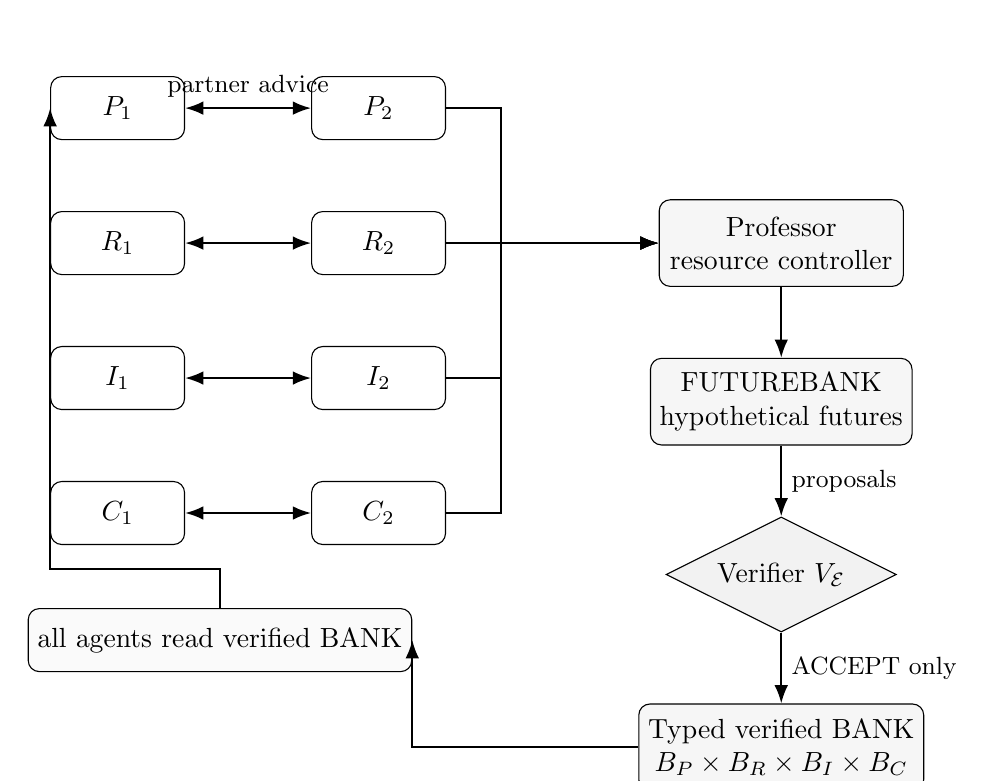
\begin{tikzpicture}[node distance=9mm and 16mm,>=Latex,
 role/.style={draw,rounded corners,minimum width=17mm,minimum height=8mm,align=center},
 box/.style={draw,rounded corners,minimum width=31mm,minimum height=11mm,align=center,fill=gray!7},
 vbox/.style={draw,diamond,aspect=2,align=center,fill=gray!10},
 bus/.style={draw,rounded corners,minimum width=42mm,minimum height=8mm,align=center,fill=gray!4},
 arr/.style={->,thick}]
\node[role] (p1) {$P_1$}; \node[role,right=of p1] (p2) {$P_2$};
\node[role,below=of p1] (r1) {$R_1$}; \node[role,right=of r1] (r2) {$R_2$};
\node[role,below=of r1] (i1) {$I_1$}; \node[role,right=of i1] (i2) {$I_2$};
\node[role,below=of i1] (c1) {$C_1$}; \node[role,right=of c1] (c2) {$C_2$};
\node[bus,below=8mm of c1,xshift=13mm] (read) {all agents read verified BANK};
\node[box,right=27mm of r2] (prof) {Professor\\resource controller};
\node[box,below=of prof] (future) {FUTUREBANK\\hypothetical futures};
\node[vbox,below=of future] (ver) {Verifier $V_{\Env}$};
\node[box,below=of ver] (bank) {Typed verified BANK\\$B_P\times B_R\times B_I\times B_C$};
\draw[<->,thick] (p1)--node[above,font=\small]{partner advice}(p2);
\draw[<->,thick] (r1)--(r2); \draw[<->,thick] (i1)--(i2); \draw[<->,thick] (c1)--(c2);
\foreach \x in {p2,r2,i2,c2}{\draw[arr] (\x.east) -- ++(7mm,0) |- (prof.west);}
\draw[arr] (prof)--(future);
\draw[arr] (future)--node[right,font=\small]{proposals}(ver);
\draw[arr] (ver)--node[right,font=\small]{ACCEPT only}(bank);
\draw[arr] (bank.west) -| (read.east);
\draw[arr] (read.north) -- ++(0,5mm) -| (p1.west);
\end{tikzpicture}
\caption{Eight-agent paired architecture. Partner and controller communication may be heuristic; only verifier-accepted material enters the shared mathematical BANK.}
\end{figure}

\section{The typed verified BANK}

Write
\[
\Bank_t=(B_{P,t},B_{R,t},B_{I,t},B_{C,t}).
\]
Each record contains at least a claim, role tag, formal scope, certificate, dependencies, provenance, verifier record, and deposit time. The BANK evolves monotonically under ordinary use:
\[
\Bank_t\subseteq\Bank_{t+1}.
\]
The inclusion is componentwise after accounting for typed metadata.

\begin{theorem}[Monotone verified memory]
Assume $\Bank_0$ contains only verifier-accepted records and every later BANK insertion requires acceptance by the same sound verifier under admissible dependencies. Then every finite $\Bank_t$ contains only certified records.
\end{theorem}
\begin{proof}
Induction on $t$. The base case is assumed. At the next step either no record is accepted, in which case the BANK is unchanged, or an accepted record is appended. Soundness of the fixed verifier gives the required validity of the new record relative to its declared dependencies.
\end{proof}

A key consequence is cross-role cooperation: a lemma discovered while trying to prove $\varphi$ may later help refute it, establish independence, or diagnose inconsistency. The roles compete over terminal settlement but cooperate through verified intermediate mathematics.

\section{FUTUREBANK: counterfactual mathematics without contamination}

The FUTUREBANK stores represented possibilities, not established theorems. A history is
\[
h=(x_0,e_1,x_1,\ldots,e_r,x_r),
\]
where each edge $e_i$ records generating action and relevant provenance. Let $\operatorname{Succ}(x)$ be a represented successor relation. Starting from root history $h_0$, define
\[
H_0=\{h_0\},\qquad
H_{d+1}=\{h\frown e\frown x:h\in H_d,\ x\in\operatorname{Succ}(\operatorname{end}(h))\},
\]
and
\[
\Future_{\le d}=\bigcup_{j=0}^d H_j.
\]
Two histories with the same visible endpoint need not be equivalent: temporary assumptions, dependency scope, path multiplicity, resource cost, and continuation rights may differ.

\subsection{Graded imagination}

It is useful to distinguish three trust grades:
\[
\Future_{\mathrm{spec}}
\longrightarrow
\Future_{\mathrm{loc}}
\longrightarrow
V_{\Env}
\longrightarrow
\Bank.
\]
The arrows indicate increasing certification, not increasing subjective confidence. A speculative branch may assume ``suppose lemma $\lambda$ can be obtained'' and explore its consequences before paying the full certification cost.

\begin{theorem}[Verifier-gated noncontamination]
Suppose speculative membership, local admissibility, compass score, controller confidence, reflection, and search history cannot bypass the fixed verifier. Then arbitrary contents of $\Future_{\mathrm{spec}}$ cannot by themselves place an invalid record in $\Bank$.
\end{theorem}
\begin{proof}
Every route into the BANK passes through the verifier. Rejected or unverified speculative objects remain outside the mathematical memory.
\end{proof}

\subsection{Safe speculative backfilling}

A speculative branch may later become certifiable if its dependencies can be discharged.

\begin{theorem}[Dependency-closed promotion]
Suppose a speculative branch has a finite acyclic dependency graph with candidate lemmas $\lambda_1,\ldots,\lambda_r$ and terminal certificate $k$. If the $\lambda_i$ are verifier-accepted in a topological order after their dependencies are available, and $k$ is then verifier-accepted, the terminal result may be deposited without importing an unverified speculative premise.
\end{theorem}
\begin{proof}
Topological induction. Every promoted dependency is verified before use. The terminal certificate is checked only after its dependency closure is verified.
\end{proof}

\subsection{Safe quotienting}

Because $|\Future_{\le d}|$ may grow as $1+b+\cdots+b^d$, compression is unavoidable at nontrivial branching factors. Let $M(h)$ be a descriptor of history $h$.

\begin{definition}[Future-sufficient descriptor]
$M$ is future-sufficient for a declared task if $M(h_1)=M(h_2)$ implies equality of all continuation information relevant to the task's legal transition, verification, resource, provenance, and counting semantics.
\end{definition}

If $M$ is future-sufficient and required path multiplicity/provenance is retained separately, equal-$M$ histories may share downstream computation. Equality of visible endpoints alone is not sufficient.

\begin{figure}[ht]
\centering
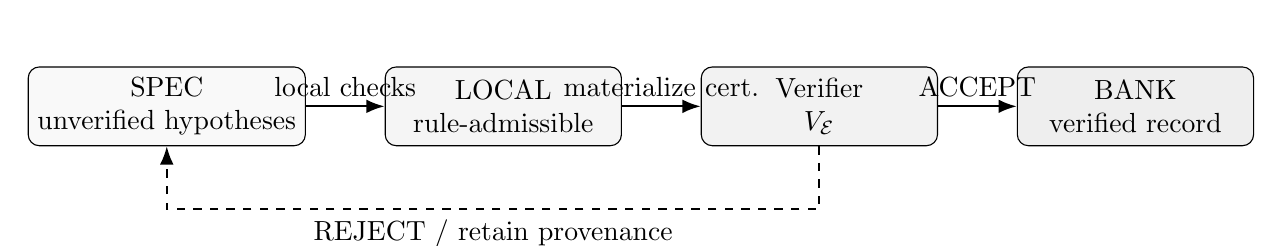
\begin{tikzpicture}[node distance=10mm,>=Latex,
 box/.style={draw,rounded corners,minimum width=30mm,minimum height=10mm,align=center},
 arr/.style={->,thick}]
\node[box,fill=gray!5] (spec) {SPEC\\unverified hypotheses};
\node[box,right=of spec,fill=gray!8] (local) {LOCAL\\rule-admissible};
\node[box,right=of local,fill=gray!10] (v) {Verifier\\$V_{\Env}$};
\node[box,right=of v,fill=gray!13] (b) {BANK\\verified record};
\draw[arr] (spec)--node[above]{local checks}(local);
\draw[arr] (local)--node[above]{materialize cert.}(v);
\draw[arr] (v)--node[above]{ACCEPT}(b);
\draw[->,dashed,thick] (v.south) -- ++(0,-8mm) -| node[pos=.25,below]{REJECT / retain provenance} (spec.south);
\end{tikzpicture}
\caption{Trust ladder. FUTUREBANK membership never implies theoremhood.}
\end{figure}

\section{Settlement horizons and the exact compass}

Let $G=(V,E)$ be a directed proof/search graph and $C\subseteq V$ the certified terminal set. Define
\[
d_C(v)=\min\{m\in\N:\exists\ v=v_0\to v_1\to\cdots\to v_m\in C\},
\]
with $d_C(v)=\infty$ if no terminal is reachable.

\begin{proposition}[One-step descent]
If $0<d_C(v)<\infty$, there exists $u\in N^+(v)$ with $d_C(u)=d_C(v)-1$, and every outgoing neighbor satisfies $d_C(u)\ge d_C(v)-1$.
\end{proposition}

Define the exact compass
\[
N(v)=v\quad(v\in C),\qquad
N(v)\in\argmin_{u\in N^+(v)}d_C(u)\quad(v\notin C),
\]
with deterministic tie-breaking.

\begin{theorem}[Exact compass fixed points]
If every considered vertex has finite directed distance to $C$, then
\[
\Fix(N)=C,
\qquad
d_C(N(v))=d_C(v)-1\quad(v\notin C),
\]
and every exact-compass trajectory reaches settlement in exactly $d_C(v)$ moves.
\end{theorem}

The ideal compass is valuable even though it is unavailable on a fresh problem: on a retained solved proof DAG, reverse breadth-first search or reverse topological dynamic programming computes exact distance labels. This converts old solved searches into supervised navigation data.

\subsection{Learned compass and half-step robustness}

Let $\widehat d_C:V\to\Rplus$ be a predictor trained only from features visible at the historical state. Define
\[
\widehat N(v)\in\argmin_{u\in N^+(v)}\widehat d_C(u).
\]
Because exact unit-edge distances are integers, the following sufficient condition is strong.

\begin{theorem}[Half-step robustness]
If
\[
\sup_{v\in V}|\widehat d_C(v)-d_C(v)|<\frac12,
\]
then every nonterminal successor selected by $\widehat N$ is a true distance-minimizing successor, so $d_C$ decreases by one at every move and $\Fix(\widehat N)=C$.
\end{theorem}

The condition is not assumed to hold for present heuristic systems. In practice, pairwise ranking accuracy among available successors may be the more realistic target.

\subsection{Weighted cost-to-settlement}

If edge $e=(v,u)$ has nonnegative computational cost $c(e)$, define
\[
d_c(v)=\inf_{v=v_0\to\cdots\to v_m\in C}\sum_{j=0}^{m-1}c(v_j,v_{j+1}).
\]
Then Bellman optimality gives
\[
d_c(v)=\min_{u\in N^+(v)}\{c(v,u)+d_c(u)\}.
\]
This is closer to the operational objective: minimize expected remaining computation to certification, not merely proof-step count.

\begin{figure}[ht]
\centering
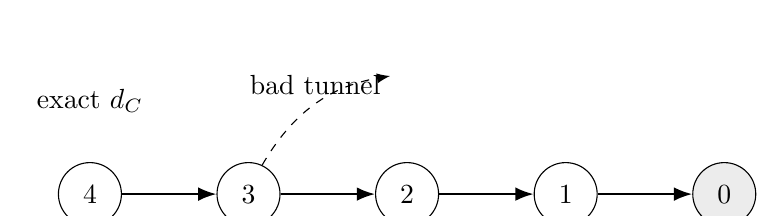
\begin{tikzpicture}[>=Latex,node distance=13mm and 12mm,
 circ/.style={circle,draw,minimum size=8mm,inner sep=1pt},arr/.style={->,thick}]
\node[circ] (v4) {4};
\node[circ,right=of v4] (v3) {3};
\node[circ,right=of v3] (v2) {2};
\node[circ,right=of v2] (v1) {1};
\node[circ,right=of v1,fill=gray!15] (v0) {0};
\draw[arr] (v4)--(v3); \draw[arr] (v3)--(v2); \draw[arr] (v2)--(v1); \draw[arr] (v1)--(v0);
\draw[->,dashed] (v3) to[bend left=25] node[above]{bad tunnel} ++(18mm,15mm);
\node[above=5mm of v4] {exact $d_C$};
\end{tikzpicture}
\caption{Ideal settlement compass: outside the certified set, the ranking decreases by exactly one.}
\end{figure}

\section{Role-specific horizons and multi-settlement geometry}

For AMLD-style search, define ideal role-specific horizons
\[
H_P(x),\ H_R(x),\ H_I(x),\ H_C(x),
\]
where each is the least resource or graph cost to an appropriate verified certificate, with $\infty$ for unreachable roles. The overall ideal settlement horizon is
\[
H_{\mathrm{AMLD}}(x)=\min\{H_P(x),H_R(x),H_I(x),H_C(x)\}.
\]
This minimum is meaningful only when the four horizons are defined under compatible cost conventions.

A directional settlement field can retain richer information:
\[
F(x)=\bigl(F_P(x),F_R(x),F_I(x),F_C(x)\bigr),
\qquad
F_P+F_R+F_I+F_C\le 1.
\]
The residual mass may represent unresolved directional information. These fields are measurements or predictions, not terminal states.

\section{Settlement tensors and the Professor controller}

A scalar density asks ``how promising is this region?'' A settlement tensor can also encode who produced the information, who can exploit it, where it arose, and which certificate class it supports. Write
\[
S_{a,b,r,c}(x)
\]
for estimated settlement value from source agent $a$, useful to recipient $b$, in region $r$, toward certificate class $c$. A decomposition is
\[
S=S^{\mathrm{direct}}+\alpha S^{\mathrm{lemma}}+\beta S^{\mathrm{transfer}}.
\]
The transfer term is where communication between couples becomes mathematically visible.

Let $u_i\ge 0$ be current resource allocated to active mode $i$, with
\[
\sum_{i=1}^n u_i=B.
\]
Let $F_x(u)$ be an estimated settlement objective. The Professor solves
\[
\max_{u\in U}F_x(u).
\]
If $U$ is compact and nonempty and $F_x$ is continuous, an optimum exists. If $U$ is convex, $F_x$ is differentiable and concave, and a suitable constraint qualification holds, KKT conditions characterize global optima. At an interior equality-constrained optimum,
\[
\frac{\partial F_x}{\partial u_i}(u^*)=\lambda
\]
for each active channel: marginal settlement value is equalized.

\subsection{Diminishing returns scheduler}

One transparent model is
\[
f_i(u_i)=w_i(1-e^{-a_i u_i}),\qquad w_i,a_i>0,
\]
so $F(u)=\sum_i f_i(u_i)$ is strictly concave. Interior coordinates satisfy
\[
w_i a_i e^{-a_i u_i^*}=\lambda,
\qquad
u_i^*=\frac1{a_i}\log\frac{w_i a_i}{\lambda}.
\]
With anti-starvation lower bounds $u_i\ge m_i$,
\[
u_i^*=\max\left\{m_i,\frac1{a_i}\log\frac{w_i a_i}{\lambda}\right\}.
\]
This is a model, not a claim that empirical settlement value is exactly exponential.

\subsection{Imperfect measurement}

Let $F$ be the true unknown allocation value and $\widehat F$ an estimate satisfying
\[
\|\widehat F-F\|_\infty\le\eps.
\]
If $u^*$ maximizes $F$ and $\widehat u$ maximizes $\widehat F$, then
\[
F(u^*)-F(\widehat u)\le 2\eps.
\]
If $F$ is $\mu$-strongly concave, this implies the allocation error bound
\[
\|\widehat u-u^*\|\le 2\sqrt{\eps/\mu}.
\]
These results explain why an imperfect but calibrated settlement tensor can still be useful.

\section{First-order and second-order compasses}

The first-order compass scores mathematical transitions:
\[
K_1(x,y)=\text{estimated value of moving from proof state $x$ to $y$}.
\]
The second-order compass scores policy actions:
\[
K_2(\State,a)=\text{estimated value of controller action $a$ in full search state $\State$}.
\]
Actions may include continuing locally, switching basins, reallocating budget across couples, changing novelty, backfilling a speculative Futurebank branch, revising control coordinates, or increasing fallback share.

The full search state can therefore be written
\[
\State_t=(\Bank_t,\Future_t,\Hist_t,\mathsf R_t,Q_t,M_t),
\]
where $\Hist_t$ is verifier/search history, $\mathsf R_t$ is reflective/self-description state, $Q_t$ is controller/resource state, and $M_t$ is pair/cross-pair communication state.

\section{Formal self-awareness as a search coordinate}

Formal self-awareness is not consciousness and is not required for ordinary counterfactual planning. A chess engine can imagine futures without formally proving facts about itself. Conversely, a machine may prove a weak self-description while having a trivial search process.

A reflection sequence may begin with
\[
\theta_0=\operatorname{ATP}(\langle M\rangle),
\qquad
\theta_{k+1}=\operatorname{Pr}(\langle M\rangle,\langle\theta_k\rangle).
\]
A tagged ATP has Level-$n$ formal self-awareness when it proves the designated $\theta_{n-1}$, with
\[
\operatorname{lev}(M)=\sup\{n\ge1:M\vdash\theta_{n-1}\}\in\{0,1,2,\ldots\}\cup\{\omega\}.
\]
Without extra hypotheses these levels need not be cumulative; self-ascribed provability can be false in deliberately weak systems. Accordingly, the architecture uses reflection only as information about search, never as evidence that a candidate proof is valid.

\begin{definition}[Futurebank-reflective ATP]
A tagged ATP is Futurebank-reflective relative to an architecture description if its language can name relevant components and it can establish designated correct self-descriptive facts about some of its verified BANK, Futurebank generator, selector/controller, compass, verifier interface, and relations among them.
\end{definition}

\begin{theorem}[Reflection-neutral verification]
If two search states have the same fixed formal environment and admissible verified BANK, then changing Futurebank, history, reflection state, communication state, controller, or compass does not change the verifier's decision on the same certificate.
\end{theorem}

The operational Level-3 question motivating recent controllers is more mundane and measurable than philosophical self-reference:
\begin{quote}
Am I putting in cost and cost and cost while obtaining little or no settlement benefit?
\end{quote}
That question leads directly to quicksand control.

\section{Controlled creativity as constrained optimization}

Creativity is placed in the search controller, not the verifier. Let a configuration be
\[
c=(c_1,\ldots,c_m)\in G_1\times\cdots\times G_m,
\]
where each $G_i$ is a declared group. Examples of controls include policy dispersion, candidate width, novelty, route independence, proof-length tolerance, lemma speculation, restart diversity, breadth allocation, retrieval diversity, and macro compilation.

For coordinates naturally constrained to $(0,1)$, use the logit-addition group
\[
x\oplus y=\sigma(\operatorname{logit}x+\operatorname{logit}y),
\]
with identity $1/2$ and inverse
\[
x^{-1}=1-x.
\]
For additive pressure parameters such as a coefficient $\beta\in\mathbb R$, the inverse is simply $-\beta$.

\subsection{Revision operator}

Let $D(c)$ be a dissatisfaction or stagnation statistic and $\tau$ a threshold. Ordinary optimization uses a local update $\Phi$ while evidence of progress remains adequate; otherwise the controller explores the group inverse:
\[
R(c)=
\begin{cases}
\Phi(c),&D(c)<\tau,\\
c^{-1},&D(c)\ge\tau.
\end{cases}
\]
Coordinatewise or partial inversion is also allowed. Crucially, the inverse is applied to \emph{controls}, not to theorem certificates.

\subsection{Protected incumbents}

Because escaping a local basin may require temporary worsening, maintain a verifier-accepted protected incumbent $q^*$. Revision explores without deleting it. A new candidate replaces the incumbent only if it is verifier-accepted and improves the declared protected objective. A lexicographic example is
\[
(\text{compressed certificate bits},\ \text{expansions},\ \text{proof steps}).
\]
A ``revision fixed point'' means only that a declared finite neighborhood produced no accepted improvement under the tested budget. It is not a proof of global optimality.

\begin{figure}[ht]
\centering
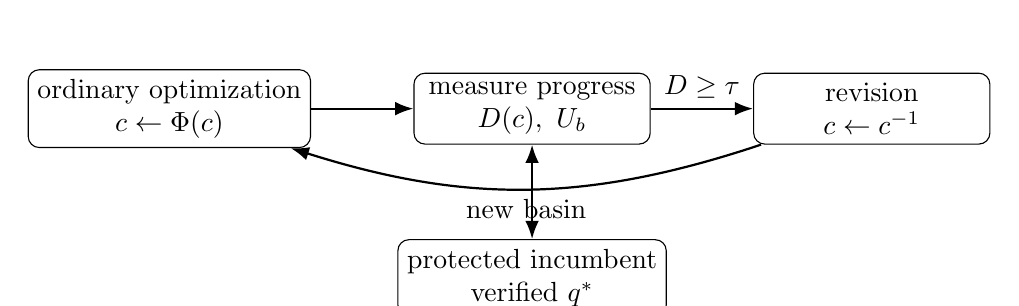
\begin{tikzpicture}[>=Latex,node distance=12mm and 13mm,
 box/.style={draw,rounded corners,minimum width=30mm,minimum height=9mm,align=center},arr/.style={->,thick}]
\node[box] (opt) {ordinary optimization\\$c\leftarrow\Phi(c)$};
\node[box,right=of opt] (measure) {measure progress\\$D(c),\ U_b$};
\node[box,right=of measure] (rev) {revision\\$c\leftarrow c^{-1}$};
\node[box,below=of measure] (bank) {protected incumbent\\verified $q^*$};
\draw[arr] (opt)--(measure);
\draw[arr] (measure)--node[above]{$D\ge\tau$}(rev);
\draw[arr] (rev) to[bend left=18] node[below]{new basin} (opt);
\draw[<->,thick] (measure)--(bank);
\end{tikzpicture}
\caption{Group-inverse revision changes the search controls while a verified incumbent remains protected.}
\end{figure}

\section{Certificate complexity: what can and cannot be minimized}

Let $q$ denote a current partial proof object and $\ell(q)$ the losslessly compressed bit length of its serialized partial certificate trail. Raw $\ell(q)$ is generally nondecreasing as proof material is appended. Therefore the naive objective
\[
\min\ell(q)
\]
is mathematically misaligned: it can prefer an empty or shallow partial proof.

Two distinct quantities should be separated.

\paragraph{Observable partial complexity.}
A normalized diagnostic can be
\[
z_\ell(q)=\log\frac{\ell(q)+1}{\operatorname{depth}(q)+1}.
\]
This may decrease even while $\ell(q)$ increases, because it measures compressed bit density per proof depth. It is a search diagnostic, not a true remaining distance to a certificate.

\paragraph{Ideal remaining certificate complexity.}
A conceptually cleaner objective is
\[
\Lambda(q)=\text{minimum additional coding cost of a valid completion from $q$},
\]
under a fixed additive coding convention. In an additive state graph,
\[
\Lambda(q)=\min_{u\in N^+(q)}\{c_\ell(q,u)+\Lambda(u)\},
\qquad \Lambda(q)=0\text{ on certified terminal states}.
\]
On a fresh problem $\Lambda$ is unknown; a learned predictor $\Lamhat$ could use $\ell(q)$, structural features, BANK/FUTUREBANK features, and historical proof DAG labels.

Thus the long-term two-coordinate compass is better expressed as
\[
\min \bigl(\widehat d_c(q),\ \Lamhat(q)\bigr),
\]
while the current quicksand controller uses $\Hhat$ and $z_\ell$ as practical signals.

\section{Quicksand: a resource/benefit definition}

A basin is not quicksand merely because $\Hhat$ is numerically low. The exact problem observed in earlier runs was a long plateau near $\Hhat\approx2.03$ with no verifier-accepted settlement. Since $\Hhat$ is not exact $H$, a low value can be a false promise.

Define a basin $b$ over a resource tranche $\Delta R$ and let useful benefit be
\[
\Delta B_b
= w_H[-\Delta\Hhat]_+
+ w_z[-\Delta z_\ell]_+
+ w_I\Delta I_{\mathrm{cert}}
+ w_C\Delta C_{\mathrm{completion}}
+ w_N N_{\mathrm{novelty}},
\]
where $\Delta I_{\mathrm{cert}}$ is sound information gain from exactification or certified horizon bounds and $\Delta C_{\mathrm{completion}}$ is direct completion evidence. Define utility
\[
U_b=\frac{\Delta B_b}{\Delta R+\eps}.
\]
A quicksand basin is operationally one for which $\Delta R$ is large while $U_b$ remains near zero over a declared window.

\subsection{Joint plateau rule}

The current 8.039-style treatment uses the simpler rule
\[
\text{no significant improvement in }\Hhat
\quad\land\quad
\text{no significant improvement in }z_\ell
\]
for a patience tranche. At that point, the controller revises two controls:
\[
\beta_\ell\mapsto-\beta_\ell,
\qquad
c\mapsto1-c,
\]
where $\beta_\ell\in(\mathbb R,+)$ is compression-density pressure and $c\in((0,1),\oplus)$ is a creativity coordinate. The inverse excursion is bounded. If benefit returns, ordinary minimization is restored; if not, the basin is blacklisted and the frontier is pruned away from that prefix.

This makes precise what ``try the opposite'' means without pretending that the certificate itself has an inverse.

\begin{figure}[ht]
\centering
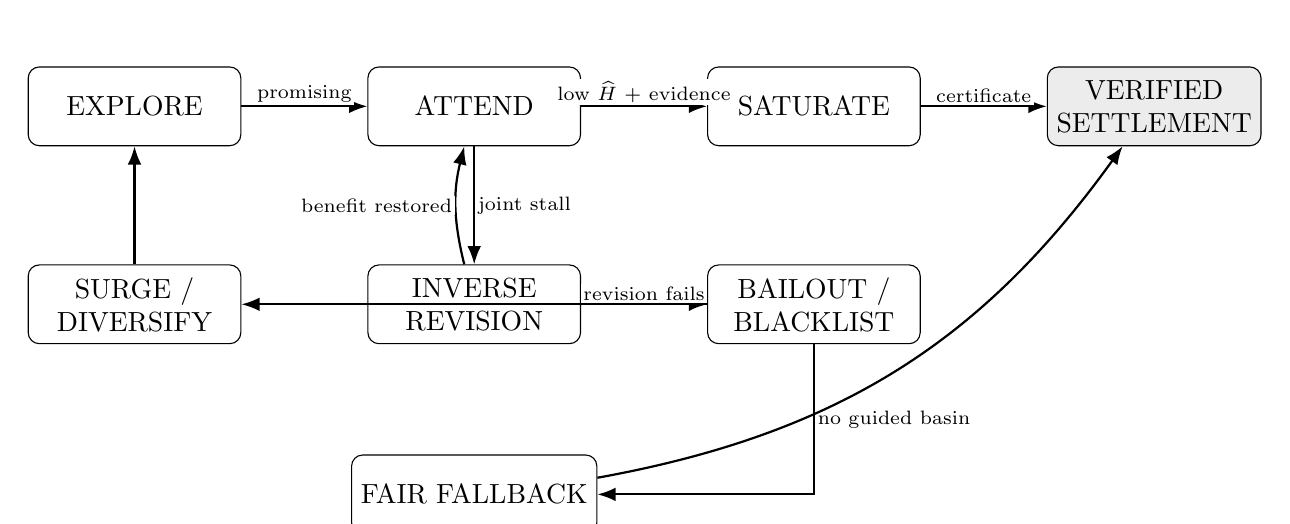
\begin{tikzpicture}[>=Latex,node distance=12mm and 16mm,
 state/.style={draw,rounded corners,minimum width=27mm,minimum height=10mm,align=center},
 arr/.style={->,thick},
 lab/.style={font=\scriptsize,fill=white,inner sep=1pt}]
\node[state] (exp) {EXPLORE};
\node[state,right=of exp] (att) {ATTEND};
\node[state,right=of att] (sat) {SATURATE};
\node[state,right=of sat,fill=gray!15] (ver) {VERIFIED\\SETTLEMENT};
\node[state,below=15mm of att] (rev) {INVERSE\\REVISION};
\node[state,left=of rev] (surge) {SURGE /\\DIVERSIFY};
\node[state,right=of rev] (bail) {BAILOUT /\\BLACKLIST};
\node[state,below=14mm of rev] (fb) {FAIR FALLBACK};
\draw[arr] (exp)--node[lab,above]{promising}(att);
\draw[arr] (att)--node[lab,above]{low $\Hhat$ + evidence}(sat);
\draw[arr] (sat)--node[lab,above]{certificate}(ver);
\draw[arr] (att)--node[lab,right]{joint stall}(rev);
\draw[arr] (rev) to[bend left=14] node[lab,left]{benefit restored} (att);
\draw[arr] (rev)--node[lab,above]{revision fails}(bail);
\draw[arr] (bail)--(surge);
\draw[arr] (surge)--(exp);
\draw[arr] (bail) |- node[lab,pos=.25,right]{no guided basin} (fb);
\draw[arr] (fb) to[bend right=22] (ver);
\end{tikzpicture}
\caption{Quicksand-aware controller. A low heuristic is not enough; saturation must be earned by continuing evidence.}
\end{figure}

\section{Current verified experiment snapshot}

The current full-toolbox \texttt{prcom} portfolio is a portfolio-level experiment: its arms collectively expose the mature tool families, but no claim is made that every arm activates every mechanism simultaneously. This avoids stacking mutually incompatible controllers into one monolithic move rule.

At the time of this article's preparation, the following verifier-gated results had been observed in the current portfolio run:
\begin{itemize}
\item A C3 controlled-creativity arm, restricted to pre-target proof mining, produced an externally verified \texttt{prcom} certificate after 41 outer expansions, with 28 proof steps and 478 compressed bits.
\item An inverse-revision experiment began from a verified key $(478,107,28)$ and accepted an inverse revision of the restart-diversity control, reaching the verified key $(470,35,28)$. A second pass found no novel verified strict improvement in the tested neighborhood, so the controller declared an \emph{experimental} fixed point at $(470,35,28)$ after two passes and 20 visited vectors. External verification accepted the emitted certificates.
\item The portfolio's ACO arm was still running at the last status check; therefore the overall workflow had not yet completed.
\end{itemize}
These numbers are experiment-specific and not claims about mathematical novelty of the theorem \texttt{prcom}, which is already a known Metamath theorem. They measure automated rediscovery/search behavior under guarded protocols.

\section{Conditional completeness and fallback}

A heuristic controller can be excellent and still miss a proof. If the chosen certificate class admits an enumerable complete fallback procedure, heuristic creativity can be interleaved with it.

\begin{definition}[Fair fallback]
A schedule is fair to fallback if the fallback enumerator receives infinitely many proposal opportunities; for example, every $q$th proposal slot for fixed $q\ge2$.
\end{definition}

\begin{theorem}[Creative conservativity under fair fallback]
Assume: (i) the verifier is fixed; (ii) fallback eventually enumerates every certificate package in its declared class; (iii) packages are submitted dependency-respectingly or revisited after dependencies are verified; (iv) fallback receives infinitely many slots; (v) accepted globally scoped BANK records do not invalidate previously valid certificates; and (vi) some finite fallback package ends in an accepting terminal certificate. Then arbitrary heuristic search, Futurebank imagination, compasses, reflection, and creativity in non-fallback slots cannot prevent eventual acceptance of that certificate.
\end{theorem}

This is a conditional liveness theorem, not a claim that every mathematical independence question has an effectively enumerable certificate class.

\section{Nonstandard analysis and K\"onig-style search arguments}

Nonstandard analysis is most useful here as theory about large finite or hyperfinite search dynamics, not as a decorative runtime ``mode.''

\subsection{Transfer of the finite compass theorem}

The finite compass theorem is uniform and first-order enough to be transferred after encoding the graph, terminal set, and successor relation internally. For an internal hyperfinite graph ${}^*G$ with internal terminal set ${}^*C$, transfer yields an internal hypernatural distance ${}^*d_C$ satisfying the same descent law on internally reachable states:
\[
{}^*d_C({}^*N(v))={}^*d_C(v)-1.
\]
If the initial distance is an unlimited hyperinteger $M$, the transferred trajectory settles after a hyperfinite number $M$ of moves, while no fixed standard finite budget need suffice. This cleanly distinguishes standard-finite settlement from hyperfinite settlement in a scaling limit.

\subsection{K\"onig's lemma interaction}

For a finitely branching rooted tree, nodes at arbitrarily large finite depths imply an infinite branch. In an NSA presentation, overspill gives a node at an unlimited hyperfinite depth $H$; its standard prefixes form an infinite standard branch when standard levels are finite.

This interacts with ranking functions as follows:
\[
\text{persistent nonsettling finite continuation}
\Rightarrow
\text{infinite/hyperfinite branch},
\]
whereas a genuine $\N$-valued rank that strictly decreases at every nonterminal move rules out such an infinite nonterminal trajectory. Thus K\"onig/NSA arguments clarify what a valid settlement rank would have to accomplish. They do \emph{not} turn a heuristic $\Hhat$ plateau into a proof of nontermination.

\section{Mathematical consistency audit}

Before launching a long experiment, the following distinctions must be enforced.

\begin{enumerate}[label=\textbf{C\arabic*.},leftmargin=2.6em]
\item \textbf{$\Hhat$ is not exact $H$.} A value such as $2.03$ is a heuristic measurement. It does not certify distance two, proximity, or theoremhood.
\item \textbf{Settlement means verifier acceptance.} A closed-looking state or $\Hhat=0$ is only a candidate until the certificate passes the verifier.
\item \textbf{Raw partial certificate length is not a descent objective.} $\ell(q)$ can grow legitimately while a proof progresses. The current treatment uses $z_\ell$ only as a secondary diagnostic; the theoretically cleaner target is remaining certificate complexity $\Lambda$.
\item \textbf{Group inversion acts on controls, not certificates.} Certificates do not naturally form a group. The inverse is applied to coordinates such as creativity or compression pressure.
\item \textbf{Revision fixed point is local and experimental.} ``No accepted improvement in this tested inverse neighborhood under this budget'' does not imply global optimality.
\item \textbf{Independence is not failure of $P$ and $R$.} Timeout or long search failure cannot certify $I$.
\item \textbf{Contradiction must remain an integrity role.} Otherwise $C$ can collapse into the refuter in classical logic.
\item \textbf{FUTUREBANK is not mathematics.} Speculative nodes, even if locally coherent, remain quarantined until dependency-closed verifier acceptance.
\item \textbf{Endpoint equality is not enough for Futurebank quotienting.} Provenance, temporary assumptions, resource obligations, and continuation rights may matter.
\item \textbf{Pair communication is epistemically typed.} Heuristic partner advice may affect selection but cannot silently become a proof premise; verified cross-pair transfer flows through BANK.
\item \textbf{KKT/global optimization claims are conditional.} Concavity, convex feasible sets, differentiability, and constraint qualifications must be stated when invoked.
\item \textbf{Fallback completeness is conditional.} It depends on a genuinely complete enumerator for the declared certificate class and a fair schedule.
\item \textbf{NSA transfer requires internal formulation.} Transfer to hyperfinite search does not automatically prove claims about arbitrary external infinite proof graphs.
\item \textbf{Portfolio ``all tools'' is a portfolio-level claim.} Different arms expose different compatible tool families; no scientific inference should pretend that one monolithic solver used every mechanism simultaneously.
\item \textbf{Search efficiency and proof validity are separate metrics.} Better expansion counts, certificate bits, or wall time are meaningful only after verifier acceptance is held fixed.
\end{enumerate}

These corrections are not cosmetic. They determine what the long experiment is actually allowed to test.

\section{Six-hour quicksand-revision experiment}

The new long experiment should answer a narrow question:
\begin{quote}
Can a joint $\Hhat$ / certificate-density progress monitor with bounded group-inverse revision prevent a single unproductive basin from consuming a six-hour run, while preserving the verifier boundary and improving or at least not catastrophically worsening time-to-first verified settlement?
\end{quote}

\subsection{Frozen elements}

The target, formal environment, theorem cutoff, learned model, random seed, candidate/verifier gate, proof semantics, and external certificate verifier are frozen. The target proof remains unavailable as a rule. The treatment is permitted to change search order only.

\subsection{Treatment state}

Per basin $b$, record
\[
(\text{resource},\ \Hhat_{\min},\ z_{\ell,\min},\ \Delta I_{\mathrm{cert}},\ \text{last progress},\ \text{revision count},\ \text{bailout count}).
\]
A joint stall triggers the bounded inverse excursion
\[
\beta_\ell\mapsto-\beta_\ell,
\qquad
c\mapsto1-c.
\]
If either $\Hhat$ or $z_\ell$ produces declared significant improvement during the revision window, the controller restores ordinary controls. Otherwise the basin is blacklisted and the search switches elsewhere.

\subsection{Primary endpoint}

The primary endpoint is
\[
\tau_0=\text{resource count at first externally verifier-accepted settlement}.
\]
If no certificate verifies before the six-hour wall limit, the outcome is \texttt{UNSETTLED WITHIN WALL LIMIT}. Heuristic progress alone is never promoted to success.

\subsection{Secondary endpoints}

Report revision events, basin bailouts, re-entry attempts, best $\Hhat$, best $z_\ell$, exactification information gain, frontier size, total expansions, proof steps, compressed certificate bits, wall time, and independent verifier result. A six-hour wall limit is a resource cap, not a promise that the process must run the full six hours if it settles earlier.

\subsection{Interpretation}

The strongest positive result would be an independently verified certificate reached after quicksand revision, together with evidence that the controller abandoned or reversed at least one stagnant basin. A weaker but still informative result would show that the treatment repeatedly detects and exits basins that would otherwise dominate the run, even if settlement is not reached. A negative result would show many revisions/bailouts with no subsequent useful progress, indicating that escape alone is insufficient and that basin generation/diversity needs improvement.

\section{Relationship to mainstream theorem-proving practice}

The architecture should be compared cautiously with mainstream systems. Learned premise/tactic/clause guidance, proof-state embeddings, best-first search, Monte Carlo or reinforcement-learning guidance, portfolio methods, proof reuse, and exact verification are established themes. The compass view is closely related to learned proof-progress prediction, and the weighted cost formulation is a standard shortest-path/Bellman idea applied to certified settlement.

What may be scientifically interesting is not an assertion that these ingredients are individually new, but whether the combined architecture produces measurable gains from the following interactions:
\begin{enumerate}
\item cross-role verified lemma transfer among $P/R/I/C$;
\item explicit paired-agent catalysis with partner advice kept outside proof semantics;
\item Futurebank speculation followed by dependency-ordered backfilling;
\item two-level compass control over both mathematical moves and policy moves;
\item formal self-description used as controller information without reflective relaxation of verification;
\item group-inverse revision of creativity/search controls after measured stagnation;
\item joint quicksand detection based on marginal benefit rather than an attractive absolute heuristic score;
\item Professor allocation driven by settlement tensors and transfer value.
\end{enumerate}
These are experimentally testable claims. The right comparison is therefore ablation under a fixed verifier and fixed benchmark, not rhetoric about general intelligence or universal mathematical creativity.

\section{Recommended experimental ladder}

A disciplined program should add one capability at a time whenever attribution matters:
\begin{enumerate}
\item verified-only baseline;
\item shared typed BANK;
\item coupled agents without speculative Futurebank;
\item provenance-preserving Futurebank;
\item graded speculation and backfilling;
\item first-order compass;
\item second-order compass / Professor allocation;
\item tension-triggered creativity;
\item group-inverse revision;
\item certificate-density quicksand monitor;
\item formal self-model supplied to the controller;
\item fair complete fallback where a completeness claim is intended.
\end{enumerate}
Each step should report verified settlement rate, $\tau_0$, verifier calls, expansions, accepted intermediate lemmas, cross-role transfer events, pair catalysis, Futurebank depth/size, revision events, and resource share by role/basin.

\section{Conclusion}

The architecture can be summarized by a strict separation of functions:
\[
\boxed{\text{BANK = verified past}}
\qquad
\boxed{\text{FUTUREBANK = represented possible futures}}
\]
\[
\boxed{\text{COMPASS = direction}}
\qquad
\boxed{\text{PROFESSOR = resource allocation}}
\]
\[
\boxed{\text{CREATIVITY/REVISION = controlled structural deviation}}
\qquad
\boxed{V_{\Env}=\text{mathematical authority}.}
\]

The paired-agent construction adds a communication layer; settlement tensors add a resource-allocation geometry; formal self-awareness adds a reflective state coordinate; and group-valued revision gives a precise mechanism for trying an opposite search regime when measured progress collapses. The quicksand problem makes the need for these distinctions concrete: a heuristic near $2$ can remain attractive for tens of thousands of expansions without settlement. The correct response is not to reinterpret the heuristic as proof distance, nor to invert the certificate. It is to measure marginal benefit, protect verified incumbents, revise search controls, escape stagnant basins, and continue to demand an independently accepted certificate.

\begin{thebibliography}{99}
\bibitem{compass}
B. Tenneson, \emph{A Discrete Compass for Proof-Ocean Navigation: Fixed Points, Learned Distance-to-Settlement, and a Trustworthy Training Protocol}, working manuscript, August 13, 2026.

\bibitem{checks}
B. Tenneson, \emph{What Checks the Proof? Bank, Futurebank, Imagination, Compass, Verification, Controlled Creativity, and Formalized Self-Awareness}, revised working manuscript, August 21, 2026.

\bibitem{tensor}
B. Tenneson, \emph{DATA 3.0 / AMLD: Discrete Settlement Tensor Optimization}, working manuscript, August 2026.

\bibitem{depths}
B. Tenneson, \emph{Depths of Induction and Formalized Self-Awareness}, Version 46.1, July 27, 2026.

\bibitem{p8018}
B. Tenneson, \emph{Predator 8.018 Reconstruction Notes}, technical reconstruction notes, August 2026.

\bibitem{bradley}
A. R. Bradley, Z. Manna, and H. B. Sipma, ``Termination of Polynomial Programs,'' \emph{VMCAI}, 2005, pp. 113--129.

\bibitem{leike}
J. Leike and M. Heizmann, ``Ranking Templates for Linear Loops,'' \emph{TACAS}, 2014, pp. 172--186.

\bibitem{enigmawatch}
Z. Goertzel, J. Jakub\r{u}v, and J. Urban, ``ENIGMAWatch: ProofWatch Meets ENIGMA,'' 2019.

\bibitem{leanprogress}
S. Huang, P. Song, R. J. George, and A. Anandkumar, ``LeanProgress: Guiding Search for Neural Theorem Proving via Proof Progress Prediction,'' 2025.

\bibitem{boyd}
S. Boyd and L. Vandenberghe, \emph{Convex Optimization}, Cambridge University Press, 2004.

\bibitem{zinkevich}
M. Zinkevich, ``Online Convex Programming and Generalized Infinitesimal Gradient Ascent,'' \emph{ICML}, 2003.
\end{thebibliography}

\end{document}
